\documentclass[11pt]{article}

\usepackage{fancyhdr}
\usepackage{graphicx}
\usepackage{geometry}
\usepackage{lastpage}
\usepackage{titling}
\usepackage{sectsty}
\usepackage{setspace}
\usepackage{changepage}
\usepackage[shortlabels]{enumitem}
\usepackage{subcaption}
\usepackage{helvet}
\usepackage{hyperref}

\usepackage{siunitx}
\usepackage{nicefrac}
\usepackage{amsmath}
\usepackage{gensymb}
\usepackage{amssymb}
\usepackage{float}

\usepackage{listings}
\usepackage{color}
\definecolor{dkgreen}{rgb}{0,0.6,0}
\definecolor{gray}{rgb}{0.5,0.5,0.5}
\definecolor{mauve}{rgb}{0.58,0,0.82}

\lstset
{
  frame=tb,
  language=MATLAB,
  aboveskip=3mm,
  belowskip=3mm,
  showstringspaces=false,
  columns=flexible,
  basicstyle={\small\ttfamily},
  numbers=none,
  numberstyle=\tiny\color{gray},
  keywordstyle=\color{blue},
  commentstyle=\color{dkgreen},
  stringstyle=\color{mauve},
  breaklines=true,
  breakatwhitespace=true,
  tabsize=3
}

\geometry
{
  letterpaper, 
  total={175.9mm,229.4mm}, 
  top=25mm, 
  left=20mm, 
  headheight=26pt,
  voffset=12pt,
  footskip=15pt
}
\author{Daniel Sturdivant}
\author{Andrew Weir}
\title{Lab 1}
\date{February 2023}
\graphicspath{ {./media/} }

\pagestyle{fancy}
\fancyhead[R]{February 6, 2023}
\fancyhead[L]{Sturdivant, Daniel \\ Weir, Andrew}
\fancyhead[C]{MECH 6970 Intro to GPS}
\fancyfoot[C]{Page \thepage\ of \pageref{LastPage}}

\makeatletter
\def\@maketitle
{
  \null
  \begin{center}
    {\huge \@title \\}
  \end{center}
  \vskip 5mm
}
\makeatother

\sectionfont{\fontsize{16}{16}}
\subsectionfont{\fontsize{13}{13}\normalfont}
\renewcommand{\thesubsection}{\arabic{section}-\arabic{subsection}}
\renewcommand{\familydefault}{\sfdefault}
\newcommand{\solution}{\textbf{\\Solution: \\}}


%% ====================================================================== %%
\begin{document}

\maketitle
\thispagestyle{fancy}
\setstretch{1.25}
% \setlength{\parskip}{0em}
% \setlength{\abovedisplayskip}{-8pt}
% \setlength{\belowdisplayskip}{12pt}
\setlength{\parindent}{0pt}

This lab involved selecting a cache at 
\url{http://www.geocaching.com/map/beta/default.aspx}. We selected the 
\emph{Uzamaki meshiagaru} cache near the Smoothie King on College Street 
(ID: GC48DJN).
\begin{figure}[H]
  \centering
  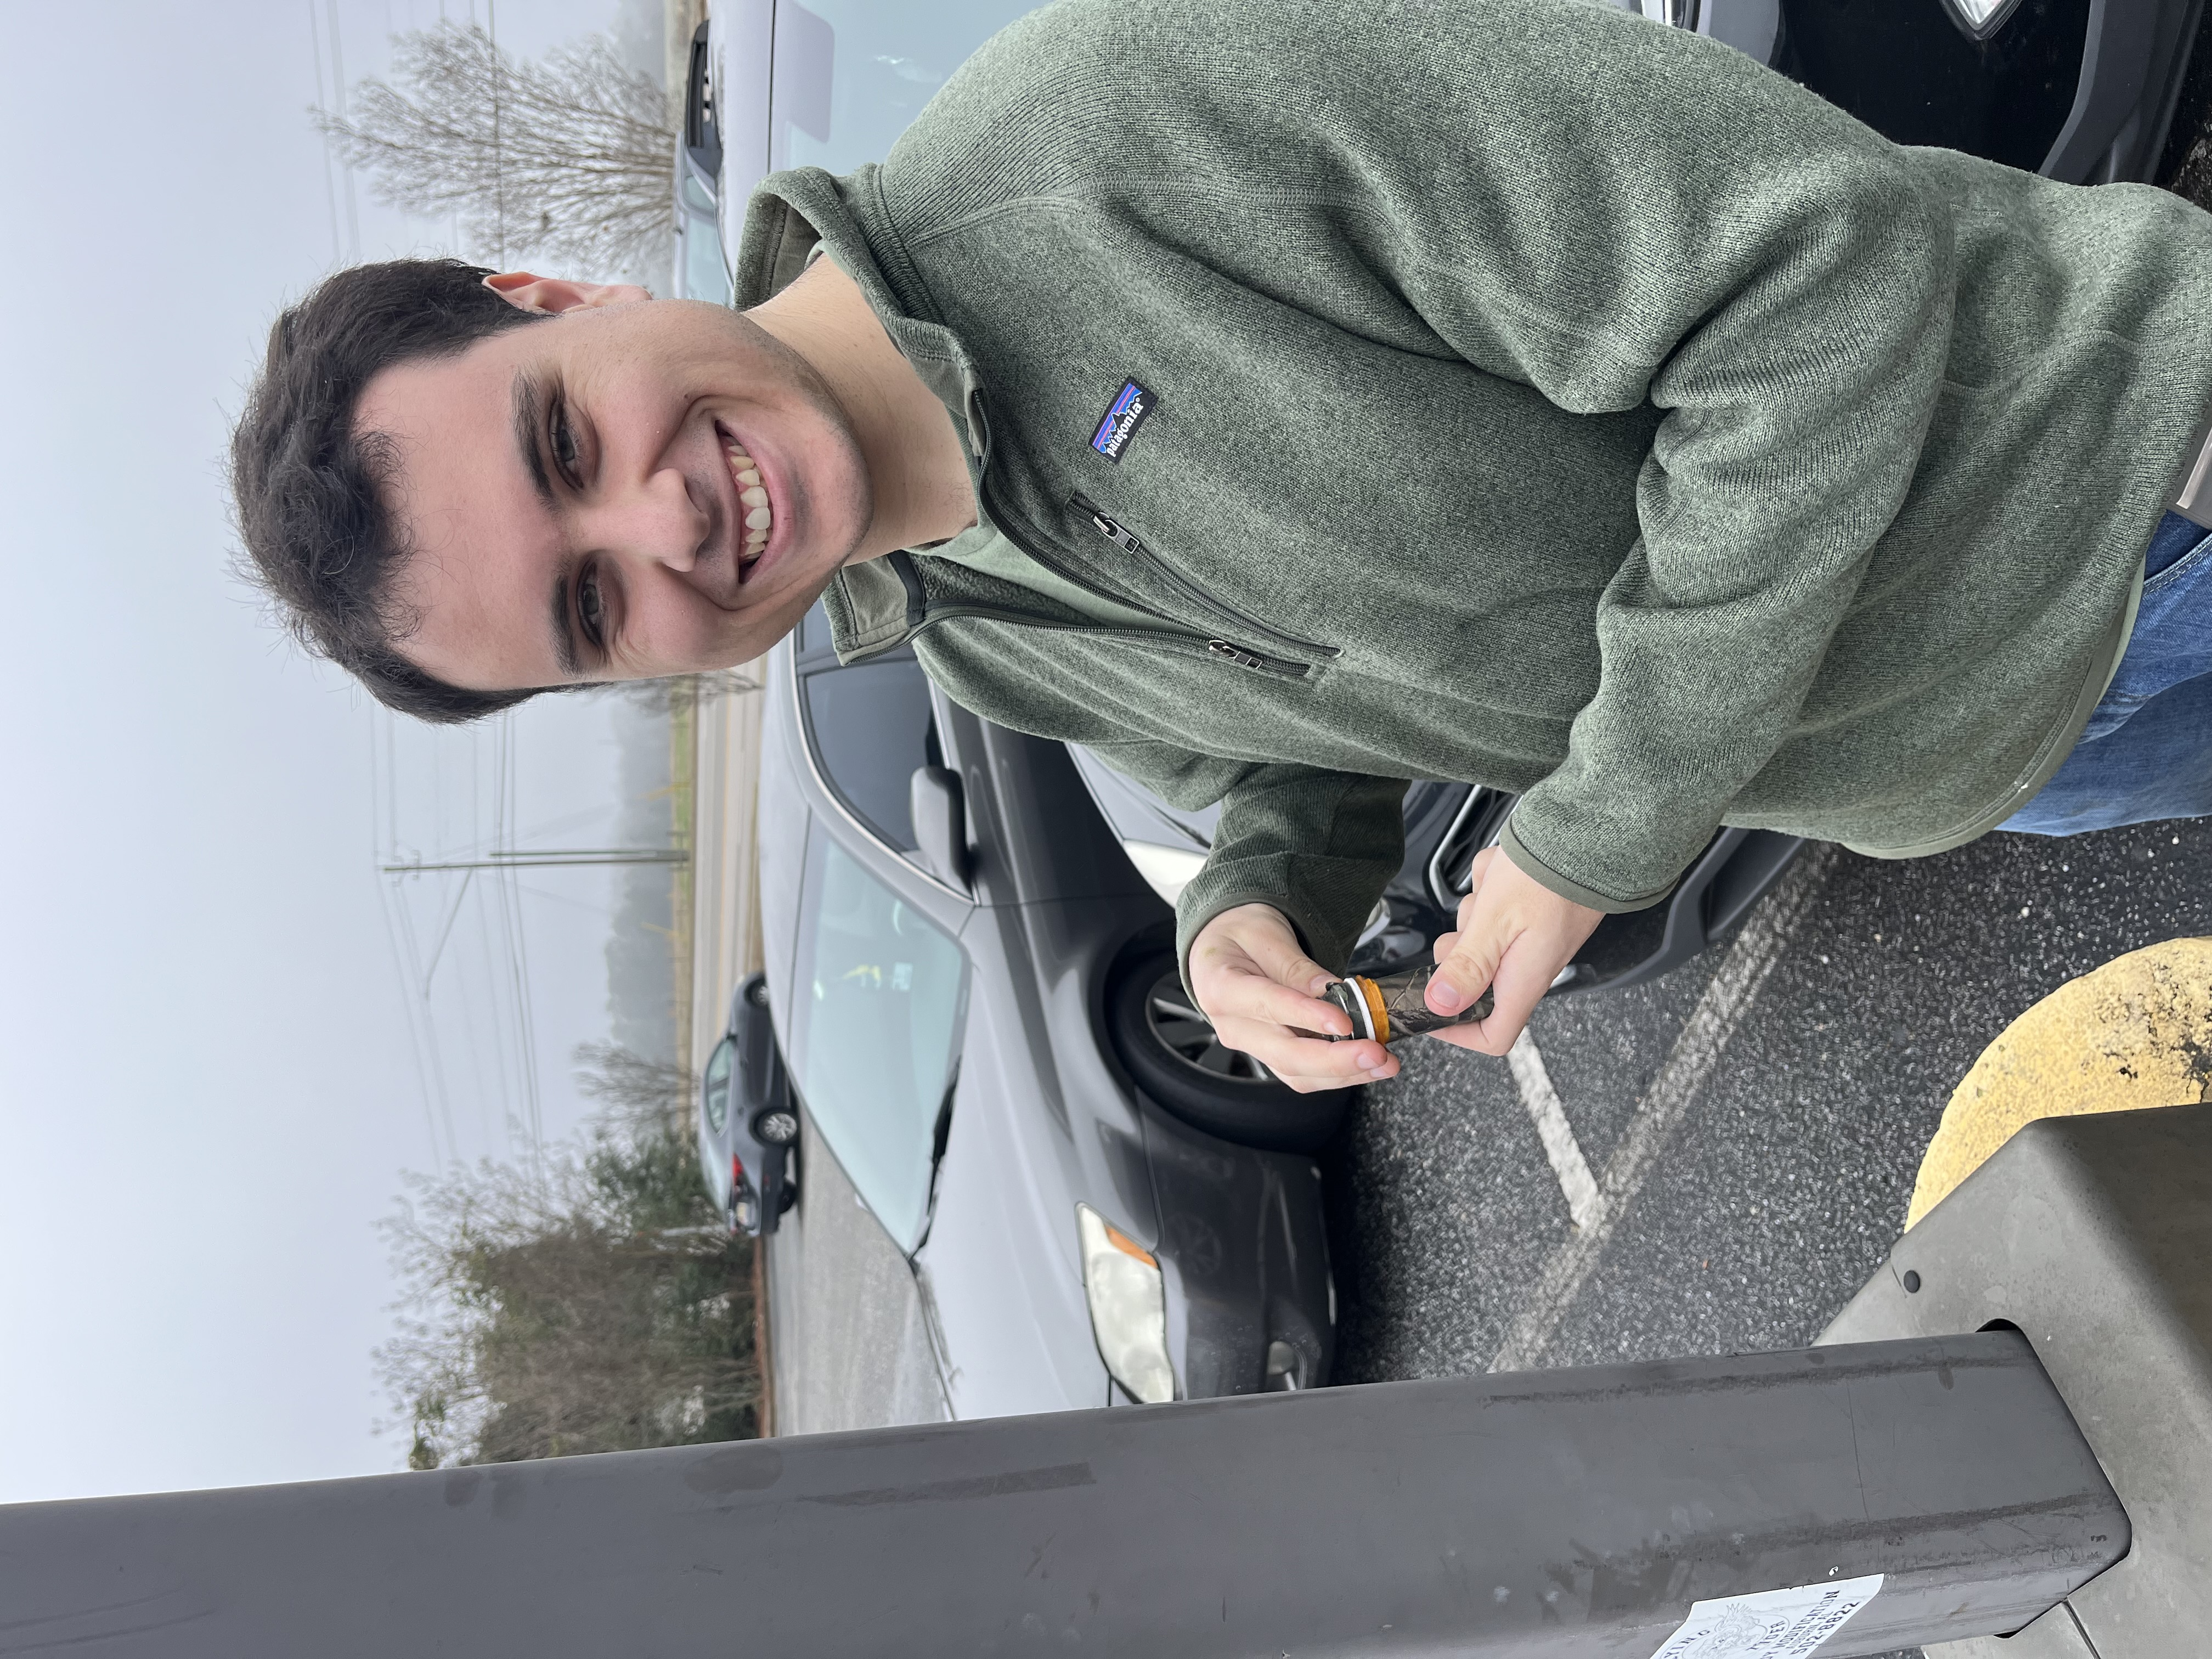
\includegraphics[angle=270,width=0.5\textwidth]{IMG_5872.jpg}
  \caption{Finding the Geocache}
\end{figure}

\begin{enumerate}[label=\textbf{\arabic*.}]
  \itemsep 36pt
  \item Note the reported coordinates of the GPS device and cache and 
  plot on a Google Maps image. Comment on the apparent accuracy of the
  plot.
  \solution
  The following coordinates were either provided by the geocache or phone:
  \begin{equation*}
    \begin{split}
      x_{cache} &=
      \begin{bmatrix}
        32.579967 & -85.495583
      \end{bmatrix}
      \\ x_{andrew} &=
      \begin{bmatrix}
        32.579981 & -85.495618
      \end{bmatrix}
      \\ x_{daniel} &=
      \begin{bmatrix}
        32.579988 & -85.495579
      \end{bmatrix}
    \end{split}
  \end{equation*}
  \begin{figure}[H]
    \centering
    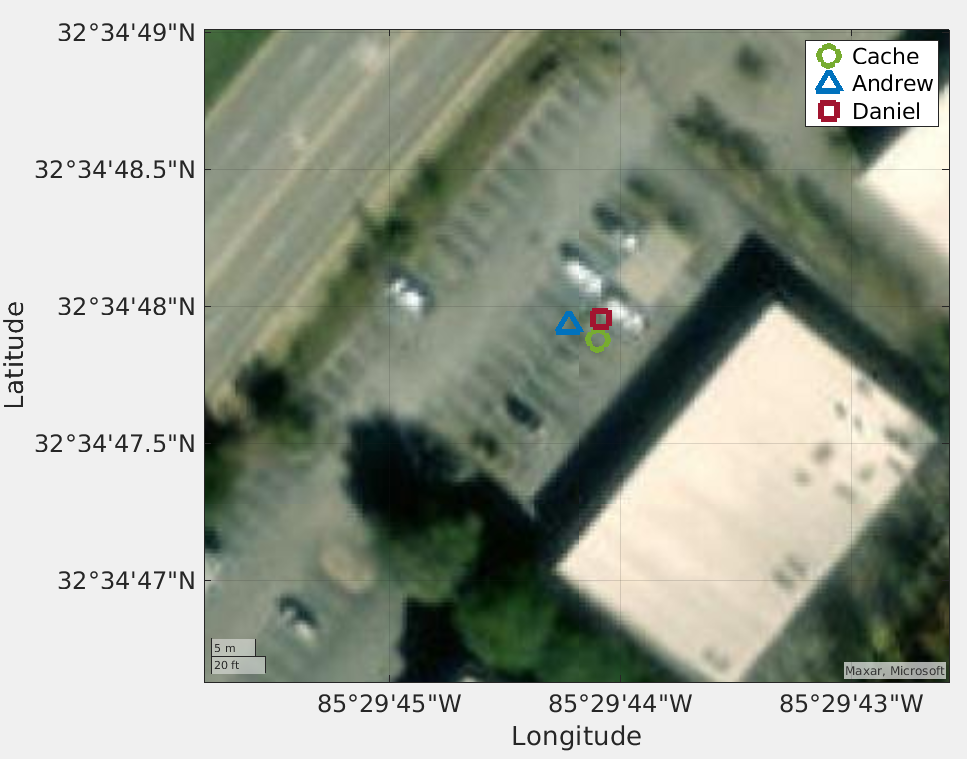
\includegraphics[width=0.7\textwidth]{p1.png}
    \caption{Geoplot of Cache and Students}
  \end{figure}
  Looking at the plot, there is only a few meters of error, which is 
  relativly accurate for a phone GPS reciever. However, a significant 
  portion of the error can be accounted for by the fact the measurements 
  were taken about a meter away from the cache. If you take the RSME of 
  the two measurements, it comes out to an error magnitude of 2.171 meters.

  \item Note the terrain, such as any tall buildings, foliage, open sky, etc. 
  \solution
  The following figures display the terrain at the cache location.
  \begin{figure}[H]
    \centering
    \includegraphics[width=0.95\textwidth]{IMG_5874.jpg}
    \includegraphics[width=0.95\textwidth]{IMG_5875.jpg}
    \caption{Terrain at Cache}
  \end{figure}
  The terrain around the cache was relatively open, as it was in a parking 
  lot. There were no tall buildings or thick foliage nearby. The tallest 
  object was the lightpost hiding the cache and a few vehicles were
  nearby. It is unlikely that these interfered with the GPS signal. The 
  most significant environmental factor was that it was very cloudy and 
  overcast day which could yield poor satellite visibility.

  \item  Note the time and day of the finding. 
  \solution
  The cache was found and measured at 11:21:27 am central time 
  on January 31, 2023.

  \item Either sketch or photograph the current satellites used by the 
  receiver.
  \solution
  The following figure shows the GNSS satellites in view and their relative 
  signal strength.
  \begin{figure}[H]
    \centering
    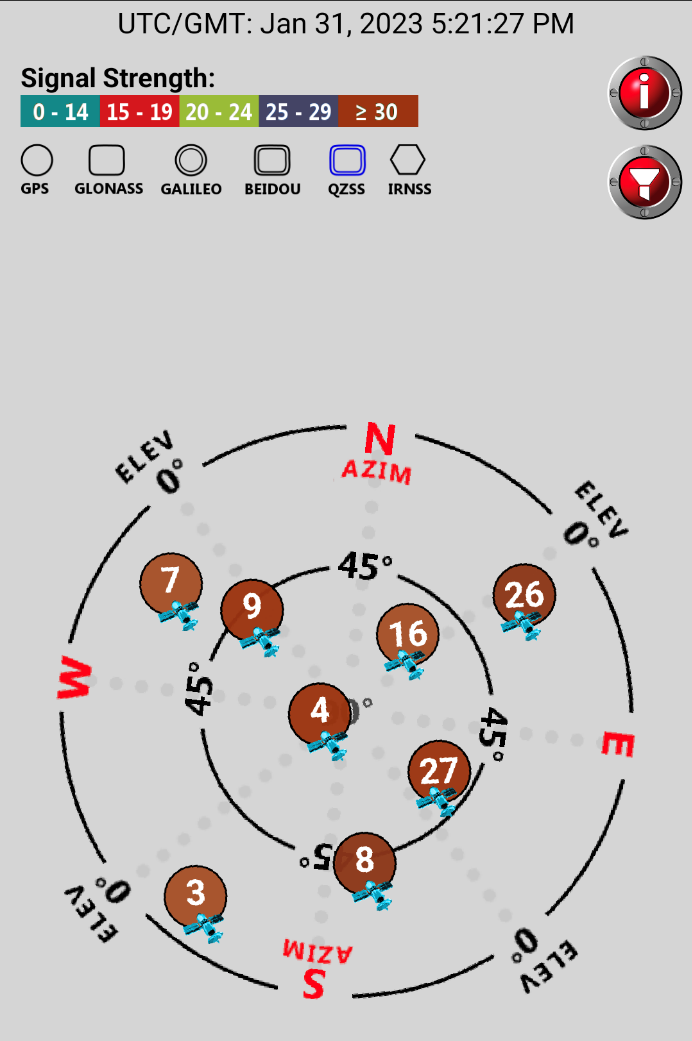
\includegraphics[width=0.5\textwidth]{p4.png}
    \caption{Phone Satellites in Use.}
  \end{figure}
  As shown, each of the 8 satellites in use have high signal strength.

  \item  Using your location and time, compare the satellite positions to the 
  receivers satellite positions using \url{https://www.gnssplanning.com} or
  \url{http://gnssmissionplanning.com}. 
  \solution
  Using both websites, the satellite locations at the geocache were as 
  follows:
  \begin{figure}[H]
    \centering
    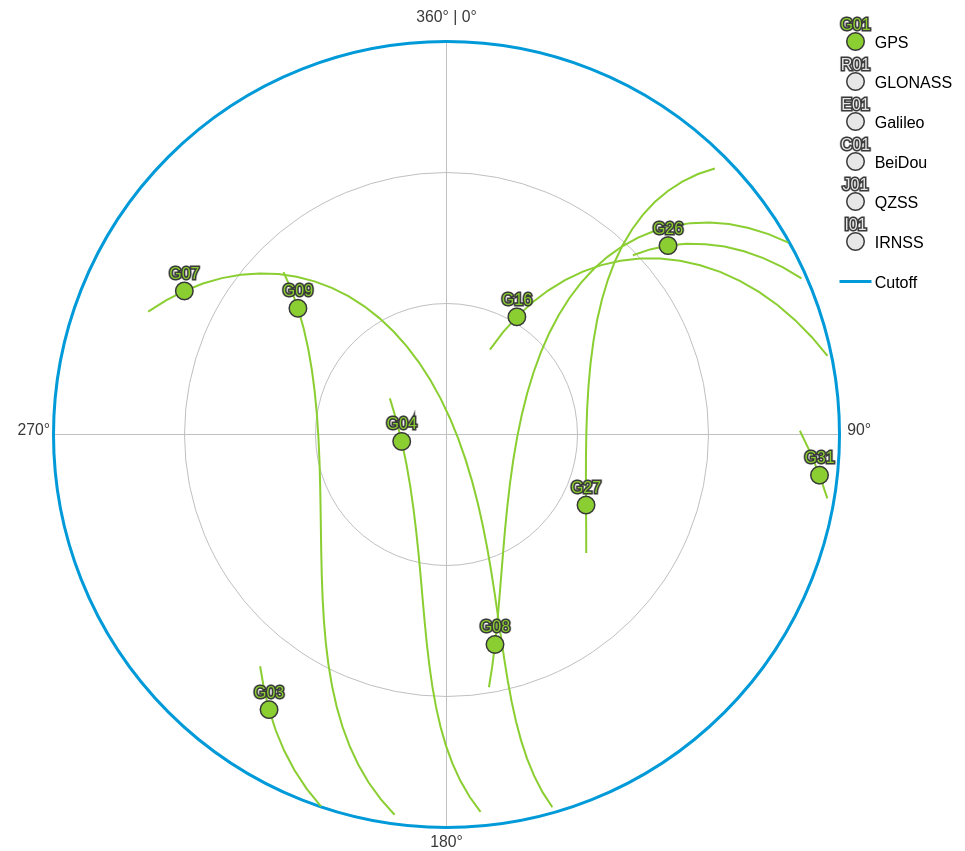
\includegraphics[width=0.5\textwidth]{trimble_sky_1120.png}
    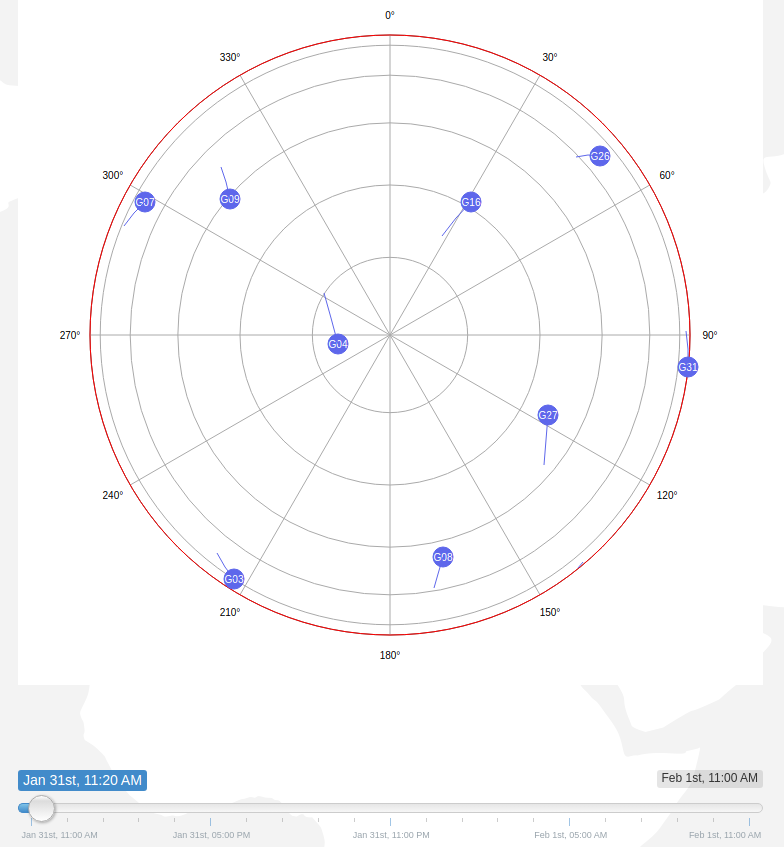
\includegraphics[width=0.5\textwidth]{mission_sky_1120.png}
    \caption{Skyplot at 11:20 am (a) Trimble (b) Mission}
  \end{figure}
  Both skyplots are nearly identical and include 9 satellites at a 0 degree 
  elevation cutoff.

  Comparing to the phone skyplot, the only difference is that the phone 
  only has 8 satellites in use whereas there should have been 9 satellites 
  available (according tho the online skyplots). This is most likely due 
  to an elevation mask removing low elevation satellites from the solution.

  \item Record the SV positions and DOP from the mission planning website for 
  time of the cache.
  \solution
  The following charts proved the world plot with satellite locations at 
  11:20 am central time followed by the DOP charts starting 11:00 am 
  central time. Only the satellites that were in view at the time of 
  measurement are included.
  \begin{figure}[H]
    \centering
    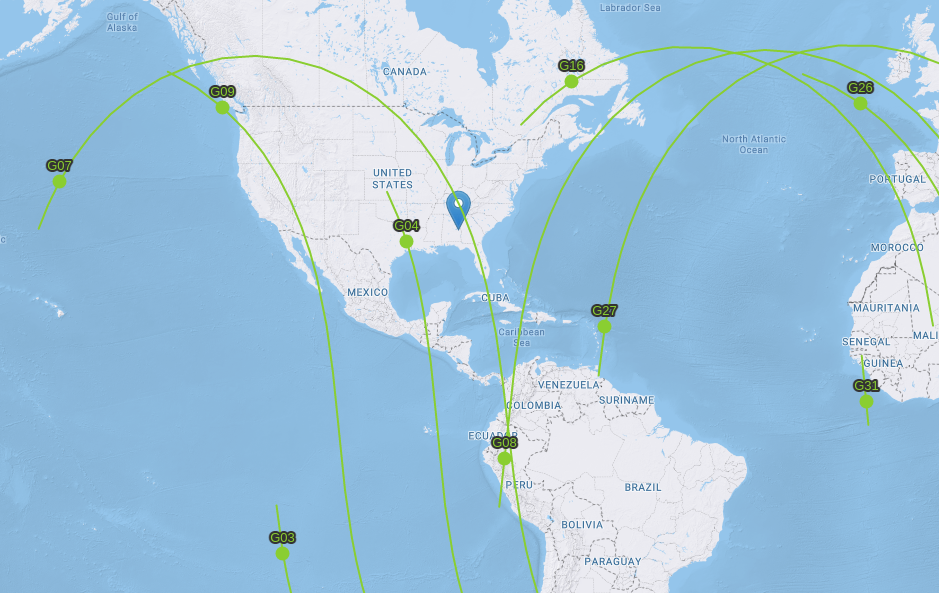
\includegraphics[width=0.7\textwidth]{trimble_world.png}
    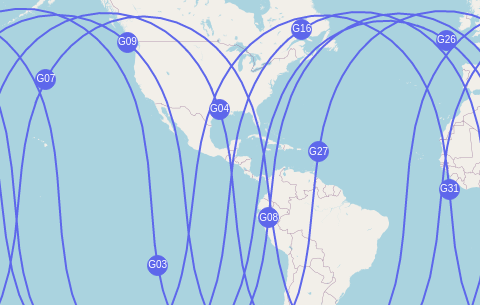
\includegraphics[width=0.7\textwidth]{mission_world.png}
    \caption{World View (a) Trimble (b) Mission}
  \end{figure}
  \begin{figure}[H]
    \centering
    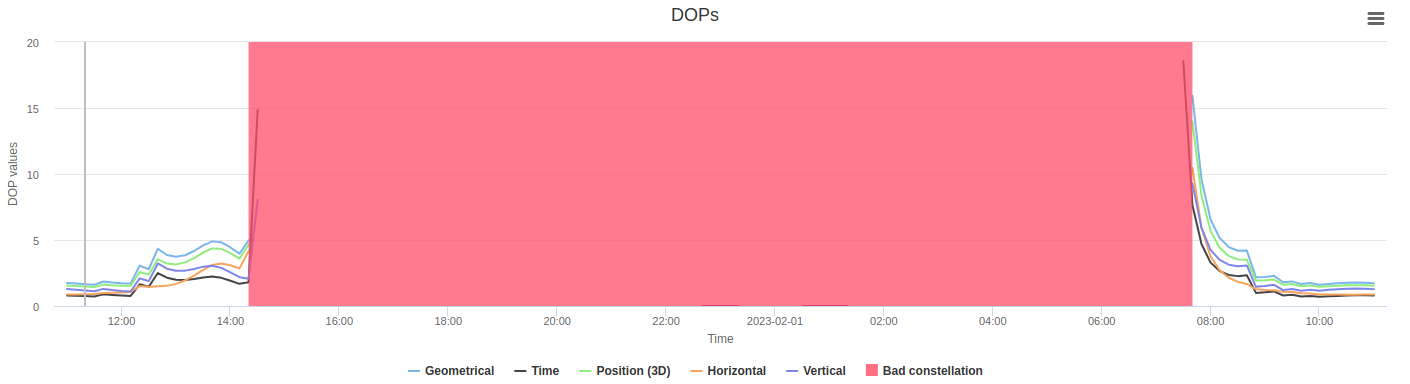
\includegraphics[width=0.9\textwidth]{trimble_dop.png}
    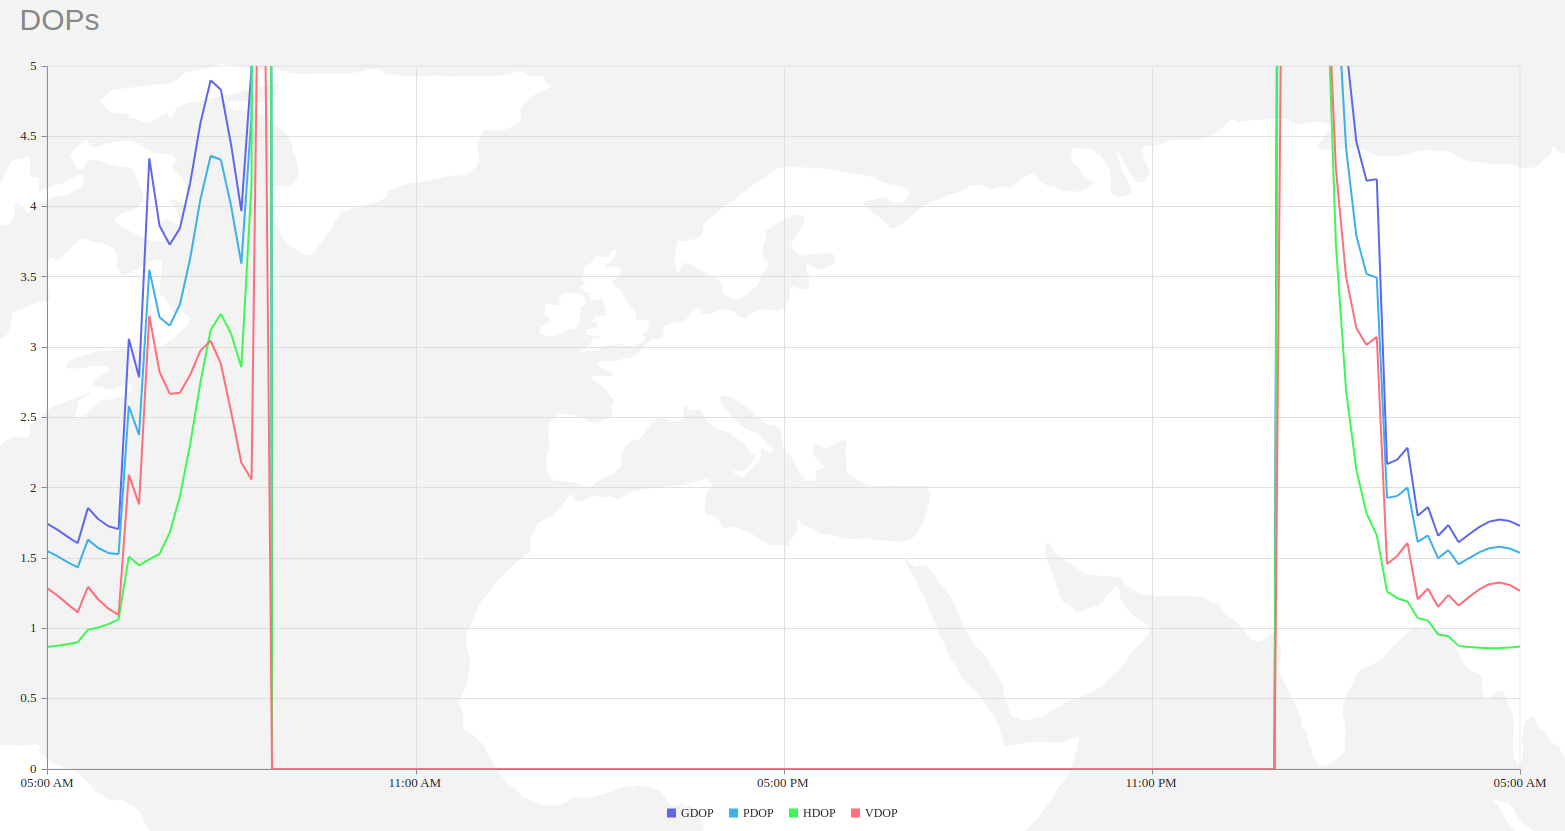
\includegraphics[width=0.75\textwidth]{mission_dop.png}
    \caption{DOP (a) Trimble (b) Mission}
  \end{figure}

\end{enumerate}

\end{document}